\documentclass{beamer}
\useoutertheme{shadow}
\usetheme{PaloAlto}
\usepackage[utf8]{inputenc}
\usepackage{graphicx}
\usepackage[ngerman]{babel}

\title{Topic 7: Vergleich von Wartestrategien \\ (Comparison of different waiting schemes)}
\author{Oliver Remy, Max Göttl, Dennis Strähhuber}
\date{\today}

\makeatletter
  \setbeamertemplate{sidebar \beamer@sidebarside}%{sidebar theme}
  {
    \beamer@tempdim=\beamer@sidebarwidth%
    \advance\beamer@tempdim by -6pt%
    \insertverticalnavigation{\beamer@sidebarwidth}%
    \vfill
    \ifx\beamer@sidebarside\beamer@lefttext%
    \else%
      \usebeamercolor{normal text}%
      \llap{\usebeamertemplate***{navigation symbols}\hskip0.1cm}%
      \vskip2pt%
    \fi%
}%
\makeatother

\begin{document}
\begin{frame}
\maketitle
\end{frame}

\begin{frame}
\tableofcontents
\end{frame}

\section{Task}
\begin{frame}
\frametitle{Task}
\textit{Es sind mittels Simulation folgende Strategien zur Organisation von wartenden Kunden zu vergleichen. In einem Bahnhof gibt es zwei Schalter für Fahrkarten. Ist es nun günstiger die wartenden Kunden in eine Warteschlange zu geben und wenn ein Schalter frei ist, wird die am längsten wartenden Kundschaft bedient. Oder ist es besser, wenn jeder Schalter eine eigene Warteschlange besitzt. Im zweiten Fall muss die Kundschaft schon bei Ankunft am Bahnhof sich entscheiden, bei welchem Schalter sie warten will. Wie sieht es aus, wenn mehr als zwei Schalter vorhanden sind? Bei der zweiten Variante kann auch überlegt werden, nach welchen Kriterien von ankommenden Kunden die Warteschlange ausgewählt wird oder auch einen eventuellen Warteschlangenwechsel beachten (wenn eine andere Warteschlange kürzer wird).\\Vergleichen Sie hier mehrere Strategien. }
\end{frame}

\section{Different Scenarios}
\begin{frame}
\frametitle{Scenario 1: One queue for $2$ or $N$ machines}
\begin{figure}
\centering
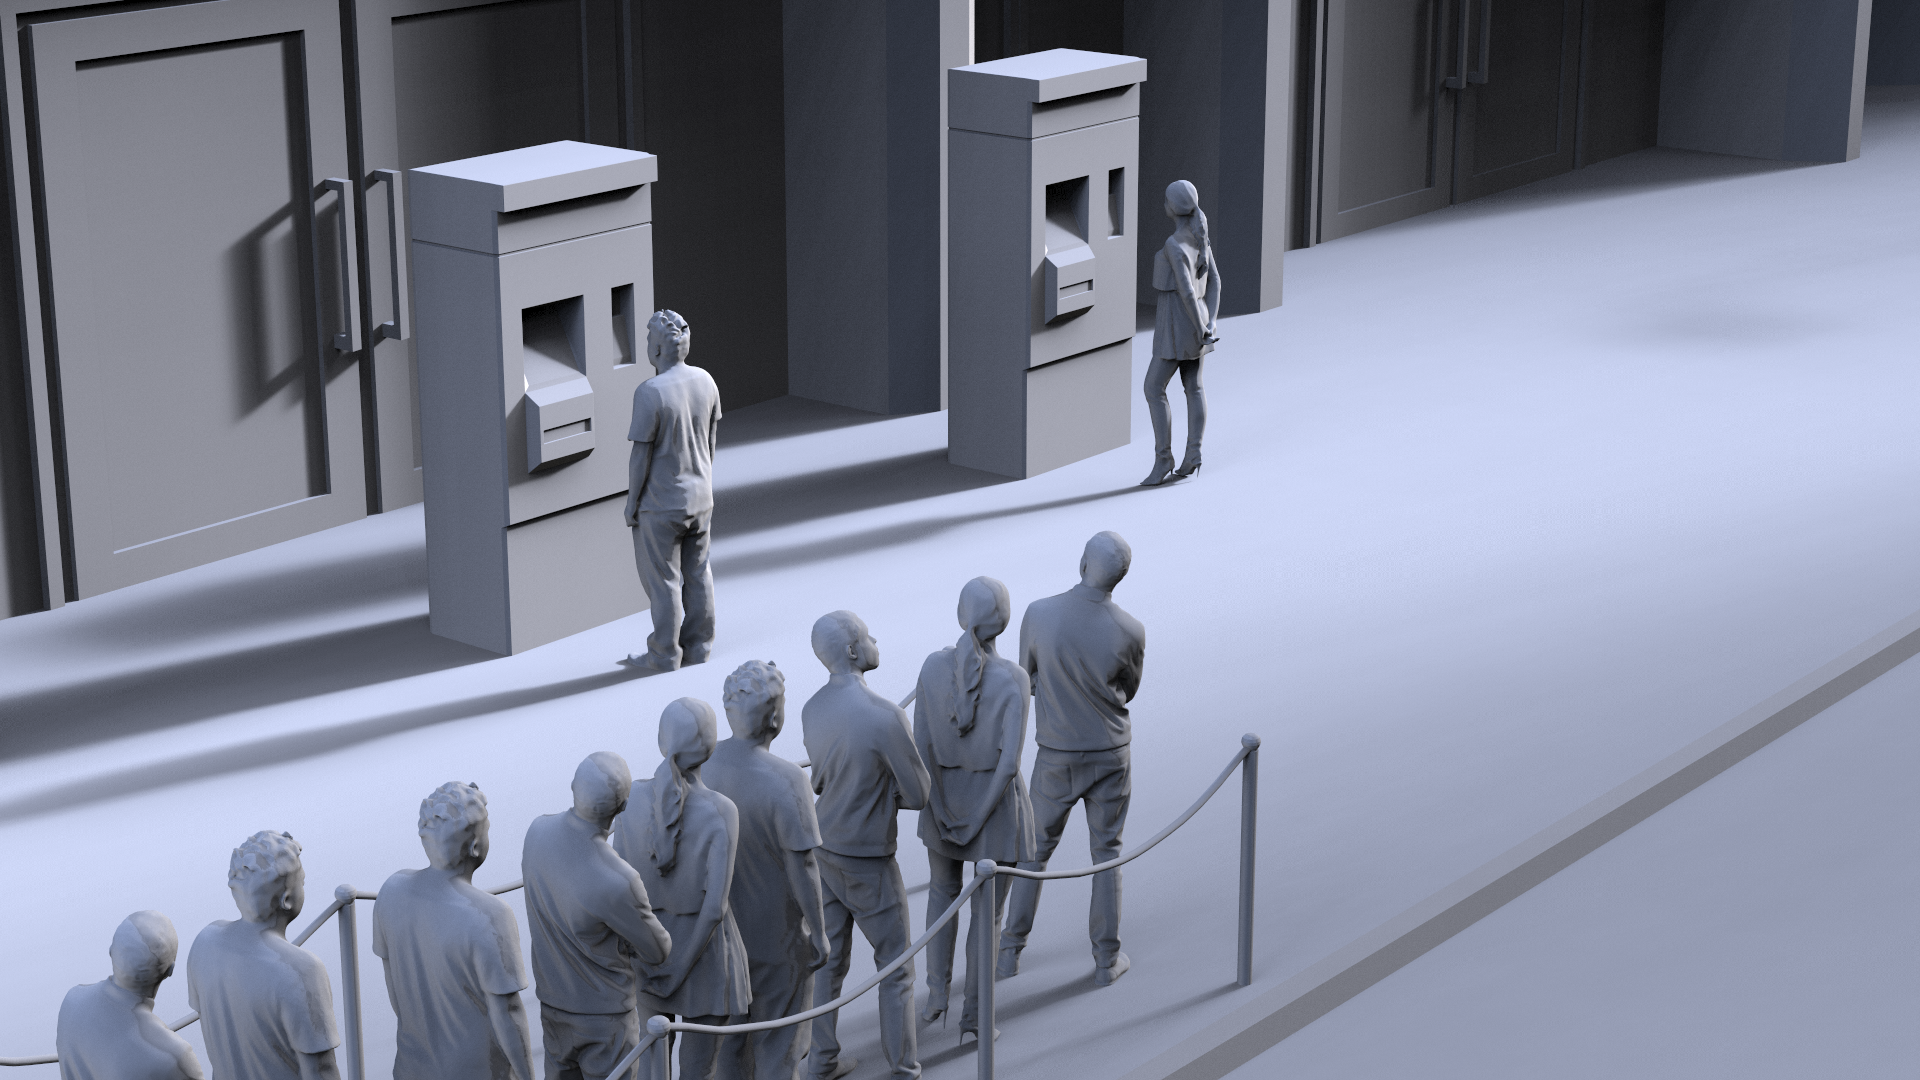
\includegraphics[width=1\textwidth]{images/scenario1.png}
\end{figure}
\end{frame}

\begin{frame}
\frametitle{Scenario 2: One queue for each of $2$ or $N$ machines}
\begin{figure}
\centering
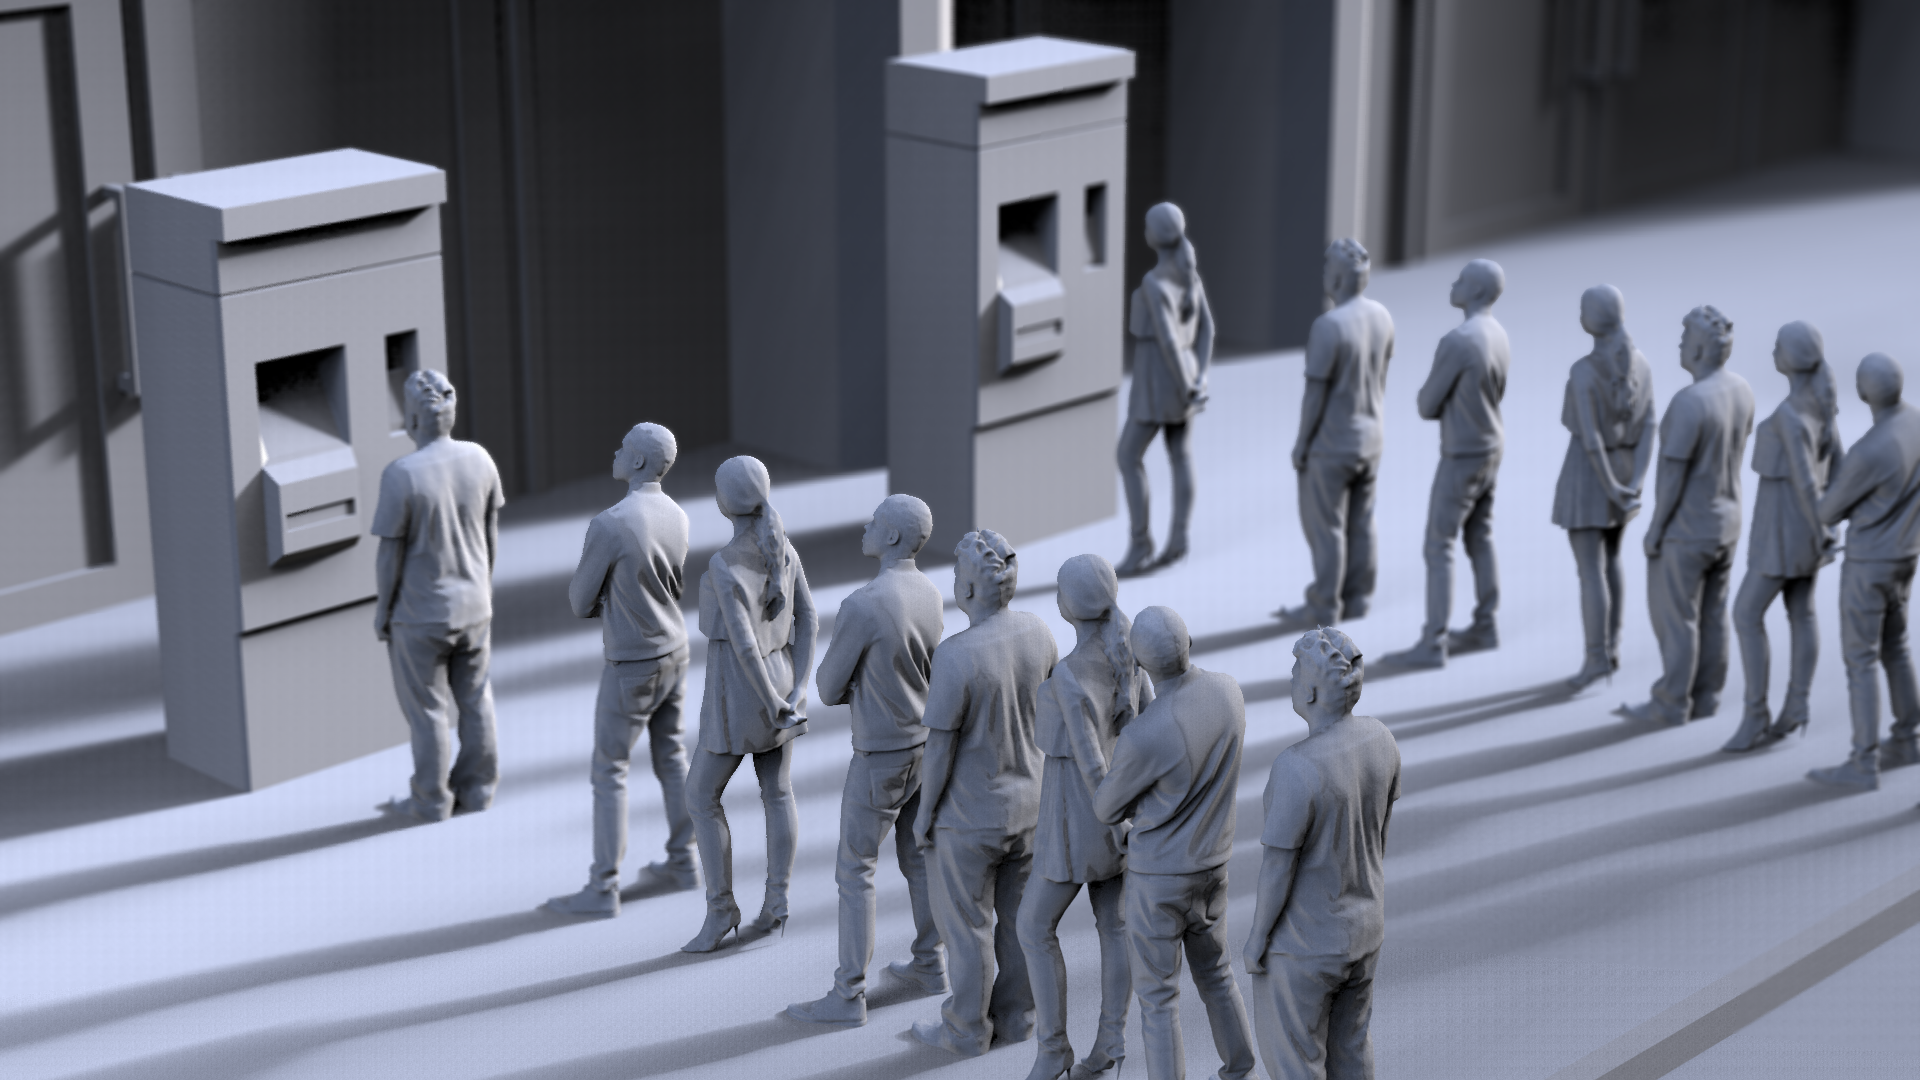
\includegraphics[width=1\textwidth]{images/scenario2.png}
\end{figure}
\end{frame}

\begin{frame}
\frametitle{Scenario 3: One queue for each of $2$ or $N$ machines}
Also one queue for each machine, but the last customer of the queue is able to switch to another queue.
\begin{figure}
\centering
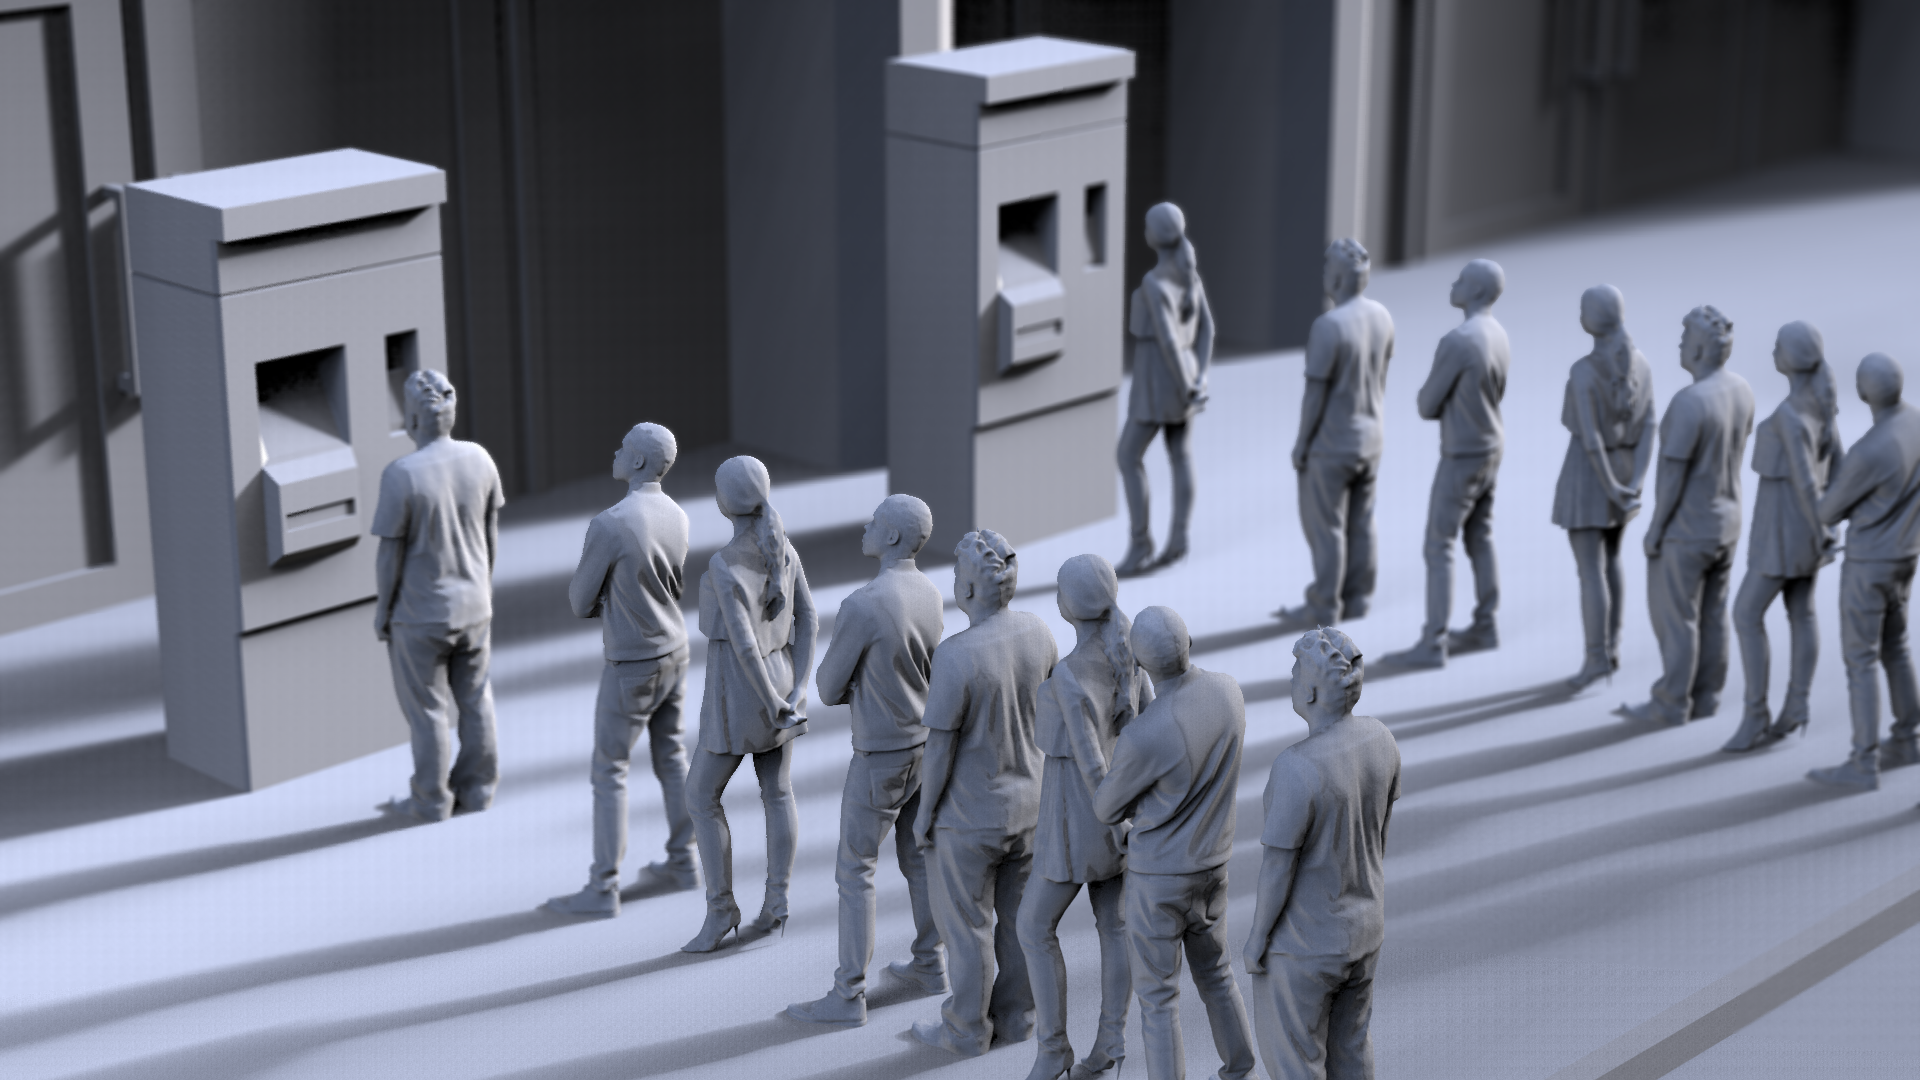
\includegraphics[width=1\textwidth]{images/scenario2.png}
\end{figure}
\end{frame}

\section{Implementation}
\begin{frame}
\frametitle{Used software and libraries}
\begin{itemize}
\item Java 8
\item 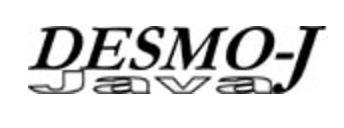
\includegraphics[width=0.2\textwidth]{images/desmoj.png} \ \url{http://desmoj.sourceforge.net/home.html}
\item 
\includegraphics[width=0.2\textwidth]{images/jfreechart.png} \ \url{http://www.jfree.org/jfreechart/}
\end{itemize}
\end{frame}

\begin{frame}
\frametitle{Event-driven modelling}
We sticked to the event-driven modelling and came up with the following events and entities:
\begin{itemize}
\item Internal events 
\begin{itemize}
\item CustomerArrivalEvent
\item CustomerFinishedEvent
\end{itemize}
\item External events
\begin{itemize}
\item NewCustomerEvent
\end{itemize}
\item Entities
\begin{itemize}
\item VendingMachine
\item Customer
\end{itemize}
\end{itemize}
\end{frame}

\begin{frame}
\frametitle{Scenario1: events}
\begin{figure}
\centering
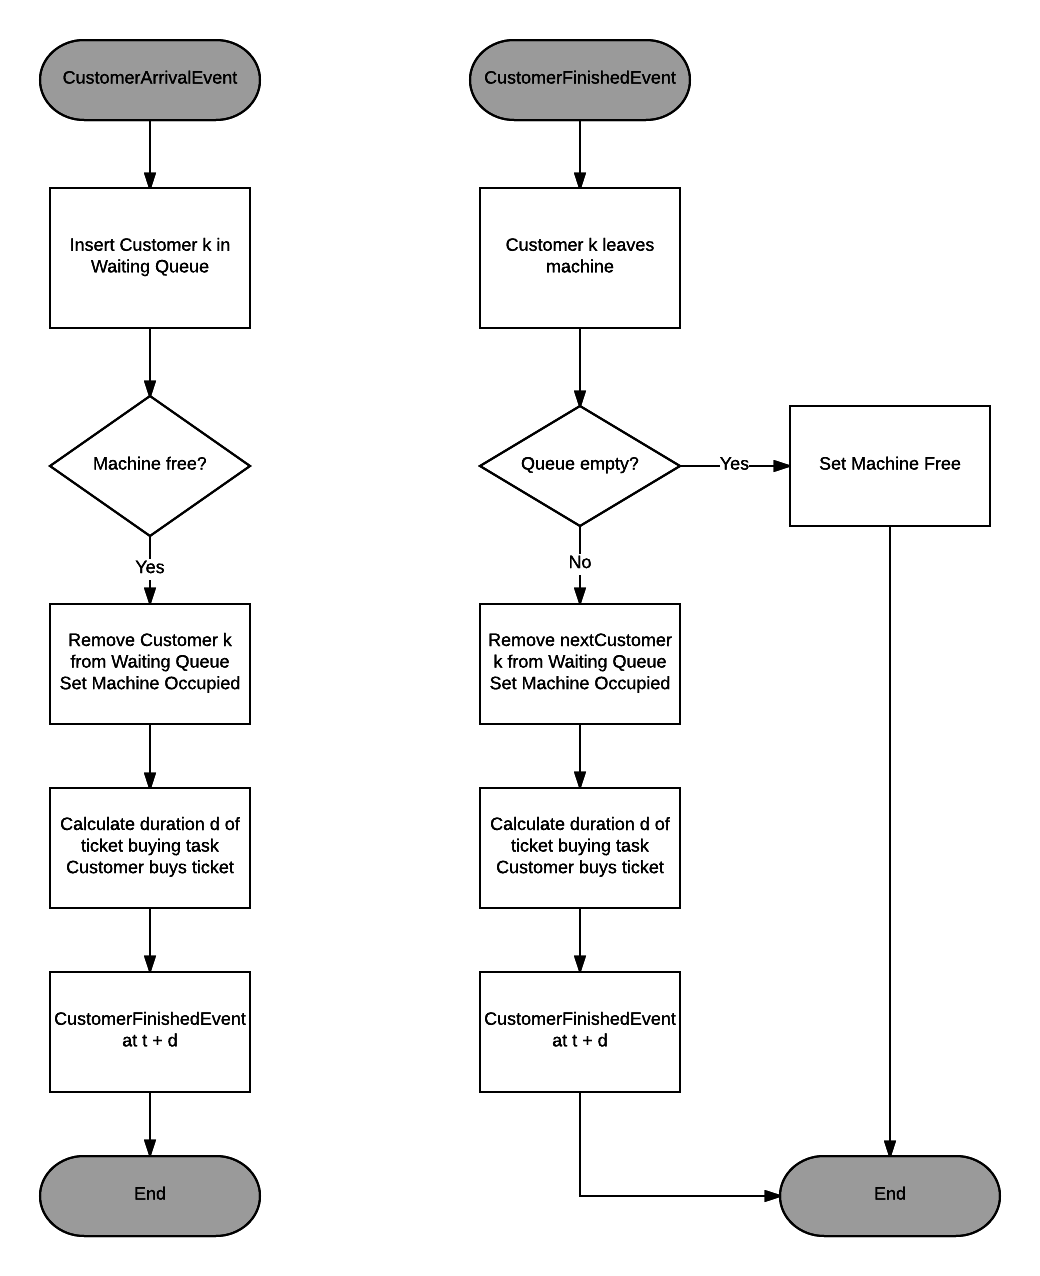
\includegraphics[width=0.57\textwidth]{images/scenario1_diag.png}
\end{figure}
\end{frame}

\begin{frame}
\frametitle{Scenario2: events}
\begin{figure}
\centering
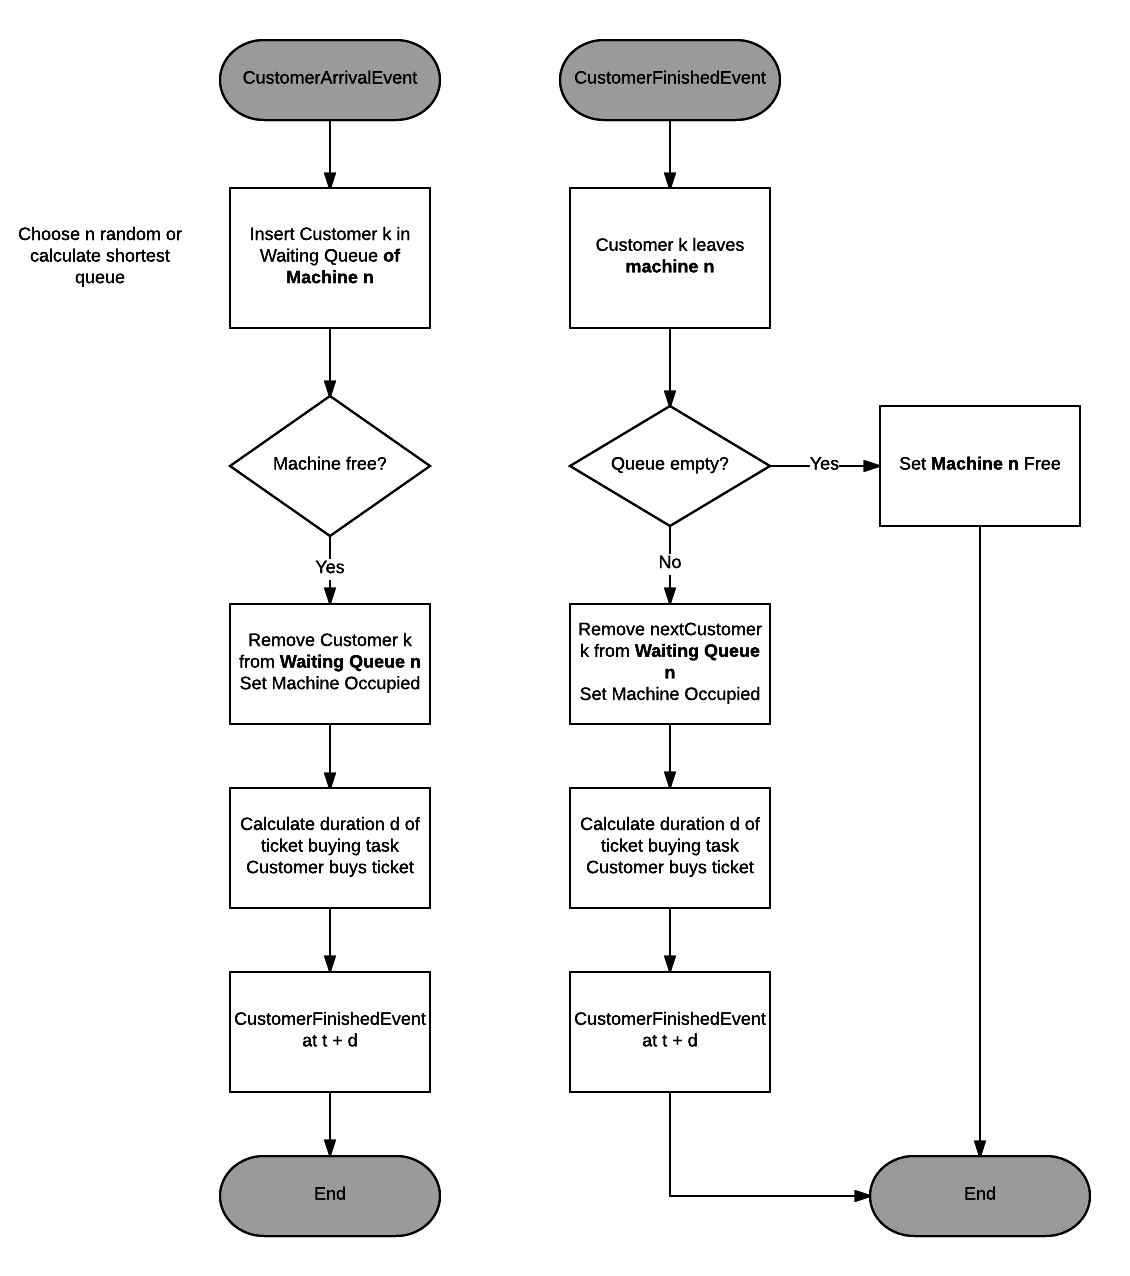
\includegraphics[width=0.62\textwidth]{images/scenario2_diag.png}
\end{figure}
\end{frame}

\begin{frame}
\frametitle{Scenario3: events}
\begin{figure}
\centering
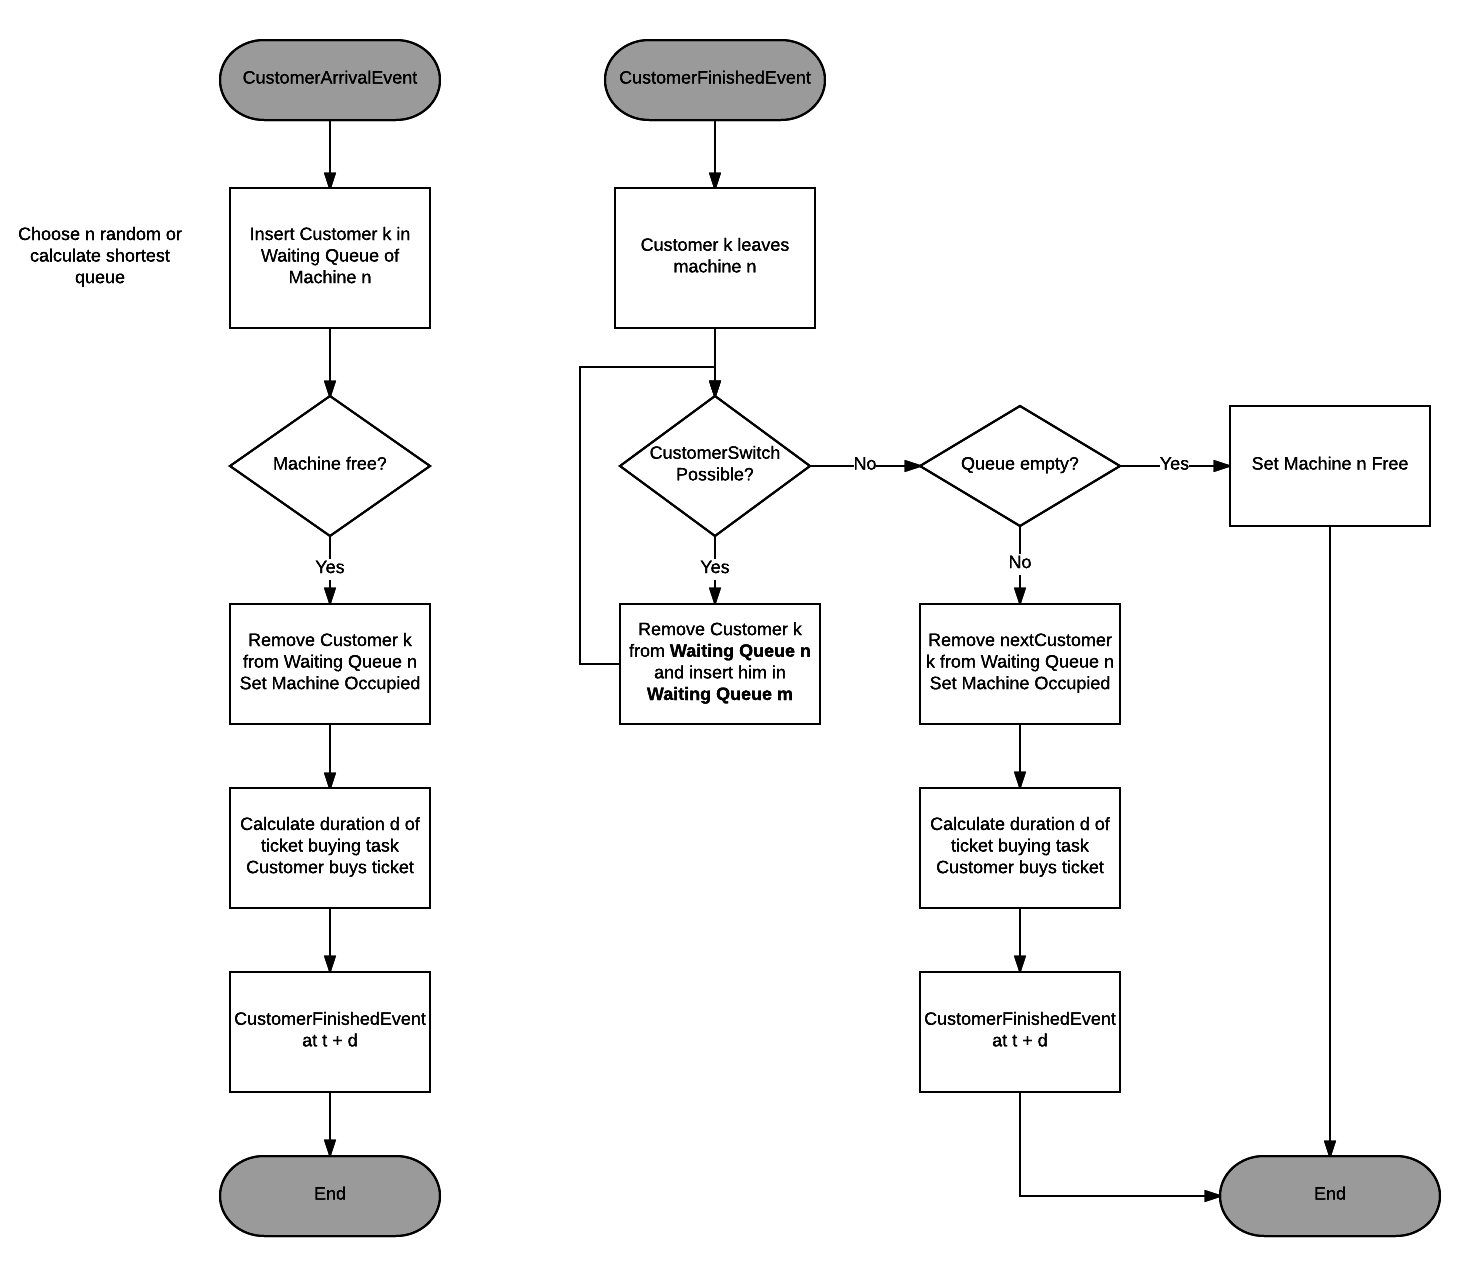
\includegraphics[width=0.8\textwidth]{images/scenario3_diag.png}
\end{figure}
\end{frame}

\section{Experiments}
\begin{frame}
\frametitle{Experiments}
We set our Distributions to the following values:
\begin{itemize}
\item CustomerDurations: Cont Uniform 0.5 - 10.0 Minutes
\item ArrivalTimeInterval: Cont Exponential 2.8 Minutes
\end{itemize}
We tested the 3 experiments with the same seed, but for different runs we took new seeds.\\
We took the following experiments with 240 Minutes of simulation:
\begin{itemize}
\item Analysis of the AVG and MAX duration of each customer in each scenario with differing number of machines
\item Assigning the new arriving customers randomly or to the shortest queue in scenario 2 and 3
\item We run 15 simulation runs for each Experiment and took the average values
\end{itemize}
\end{frame}

\begin{frame}
\frametitle{Expectations}
We expected the scenario 1 to be the perfect solution in terms of AVG and MAX duration.\\
Furthermore we expected the scenario 3 to be as good as scenario 1 when we assign new customers to the shortest queue. Scenario 2 we expected as not that effective. \\
For the random assignement of new customers we expected that scenario 2 and 3 loose more against scenario 1 as with assigning to the shortest queue.
\end{frame}

\section{Results}
\begin{frame}
\frametitle{Results shortest queue assignment, 2 machine}
\begin{figure}
\centering
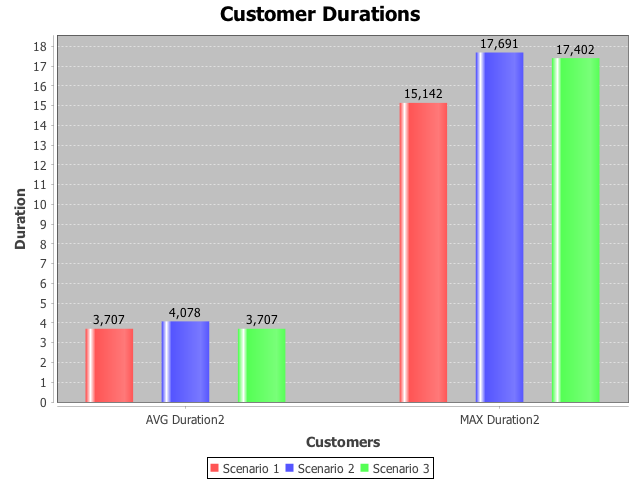
\includegraphics[width=0.93\textwidth]{results/out_2_random_false.png}
\end{figure}
\end{frame}

\begin{frame}
\frametitle{Results random queue assignment, 2 machines}
\begin{figure}
\centering
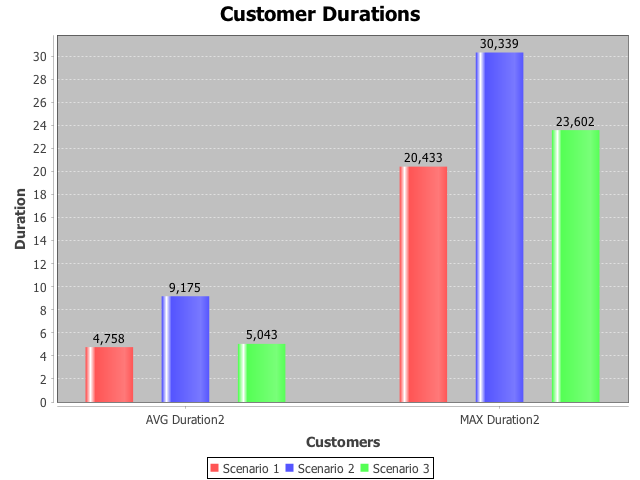
\includegraphics[width=0.93\textwidth]{results/out_2_random_true.png}
\end{figure}
\end{frame}

\begin{frame}
\frametitle{Results shortest queue assignment, varying machine}
\begin{figure}
\centering
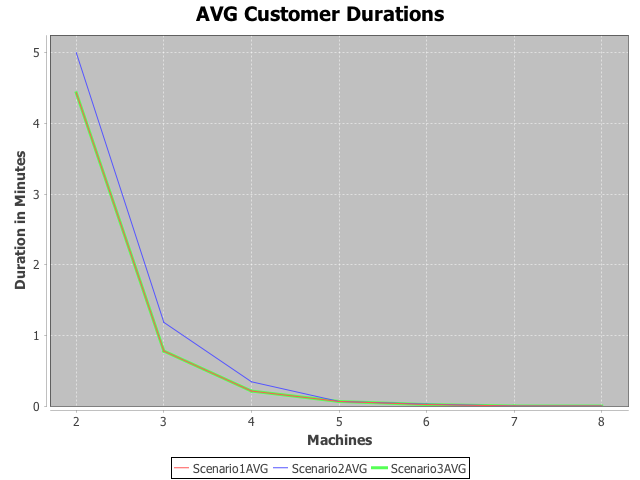
\includegraphics[width=0.93\textwidth]{results/Output_AVG_random_false.png}
\end{figure}
\end{frame}

\begin{frame}
\frametitle{Results shortest queue assignment, varying machine}
\begin{figure}
\centering
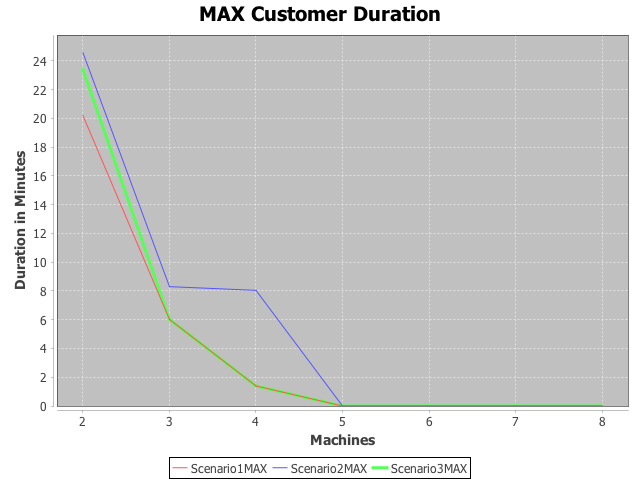
\includegraphics[width=0.93\textwidth]{results/Output_MAX_random_false.png}
\end{figure}
\end{frame}

\begin{frame}
\frametitle{Results random queue assignment, varying machine}
\begin{figure}
\centering
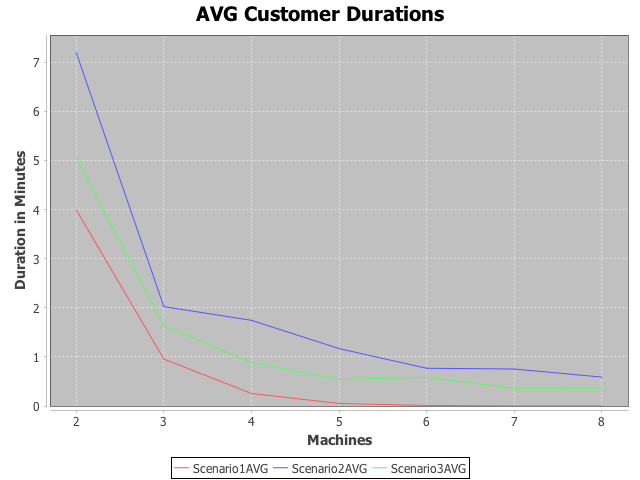
\includegraphics[width=0.93\textwidth]{results/Output_AVG_random_true.png}
\end{figure}
\end{frame}

\begin{frame}
\frametitle{Results random queue assignment, varying machine}
\begin{figure}
\centering
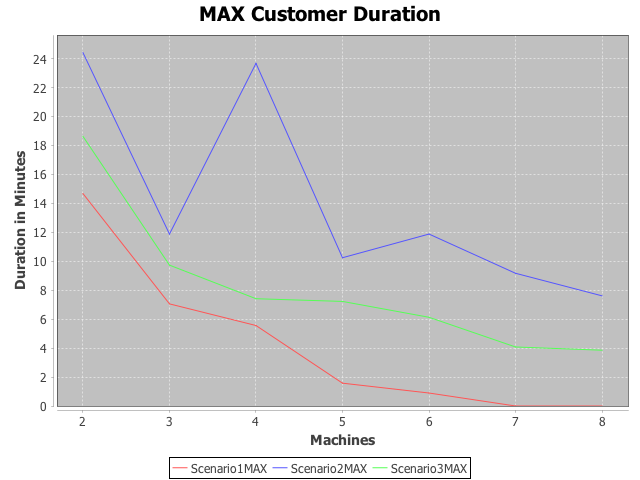
\includegraphics[width=0.93\textwidth]{results/Output_MAX_random_true.png}
\end{figure}
\end{frame}

\section{Conclusion}
\begin{frame}
\frametitle{Conclusion}
So the results were quite as expected.\\
Furthermore Scenario1 may be the fastest, but in real conditions with more machines it may be hard to manage. And we usually build queues behind each machine.
\end{frame}

\begin{frame}
\frametitle{End}
Are there any questions? \\
Thanks for your attention.
\end{frame}



\end{document}